\chapter{Conceptos fundamentales}
\label{chap:Modelo-generico}
\thispagestyle{empty}
 Para este trabajo consideramos en general tres modelos de interacción de vientos, actualmente publicado \citep{Tarango-Yong:2018a}, y anexado en esta tesis en el apéndice \ref{app:article}. Sin embargo, solamente la sección \ref{sec:fundamental-parameters} está basada en \citet{Canto:1996}. Los modelos considerados en este trabajo se describen brevemente a continuación:

\begin{itemize}
\item Una fuente localizada en el origen que emite un viento esférico con densidad isotrópica (figura \ref{fig:isotropic-aniso}, esquina superior izquierda) no acelerado que interactúa con el viento esférico isotrópico de otra fuente que se encuentra a una distancia $D$ de la primera (figura \ref{fig:crw-esquema}a). A los choques de proa resultantes se conocen como ``Cantoides''\footnote{En referencia a J. Cantó, quien encontró la solución al problema de dos vientos en la aproximación de capa delgada en \citet{Canto:1996}}. 
\item  Una fuente localizada en el origen que emite un viento esférico no acelerado cuya densidad varía como una ley de potencias de $\cos\theta$, cuyo índice denotamos como $k$, y $\theta$ es el ángulo polar de las coordenadas esféricas (figura \ref{fig:isotropic-aniso}, esquina superior derecha y páneles inferiores), que interactúa con el viento esférico isotrópico de otra fuente que se encuentra a una distancia $D$ de la primera (figura \ref{fig:crw-esquema}a). A los choques de proa resultantes se conocen como ``Ancantoides''\footnote{En inglés Ancantoid, abreviación de ``Anisotropic Cantoid''}.
\item Una fuente localizada en el origen que emite un viento esférico isotrópico no acelerado que interactúa con un viento plano paralelo no acelerado y densidad constante (figura \ref{fig:crw-esquema}b). Los choques resultantes en este caso se conocen como ``Wilkinoides''\footnote{En referencia a F.P. Wilkin, quien en \citet{Wilkin:1996} resolvió el problema de dos vientos entre un viento esférico isotrópico y un viento plano-paralelo de densidad uniforme en la aproximación de capa delgada. El término fue acuñado en \citet{Cox:2012} y en este trabajo fue adoptado.}.
\end{itemize}
Para caracterizar al choque de proa utilizaremos coordenadas esféricas, siguiendo la simetría del viento interior. La forma del choque de proa medido a partir del origen es $R(\theta, \phi)$, donde $\theta$ y $\phi$ son el ángulo polar y azimutal, respectivamente. Asumiendo simetría cilíndrica en el sistema, esta función se simplifica a $R(\theta)$, y la forma del choque se puede representar con una curva bidimensional, donde el ángulo azimutal $\phi$ es constante. De esta manera, la forma del choque en coordenadas cartesianas se obtiene mediante la conocida tranformación de coordenadas polares a cartesianas:

\begin{align}
  x &= R(\theta)\cos\theta \label{eq:polar-to-x}\\
  y &= R(\theta)\sin\theta \label{eq:polar-to-y}
\end{align}

\begin{figure}
  \centering
  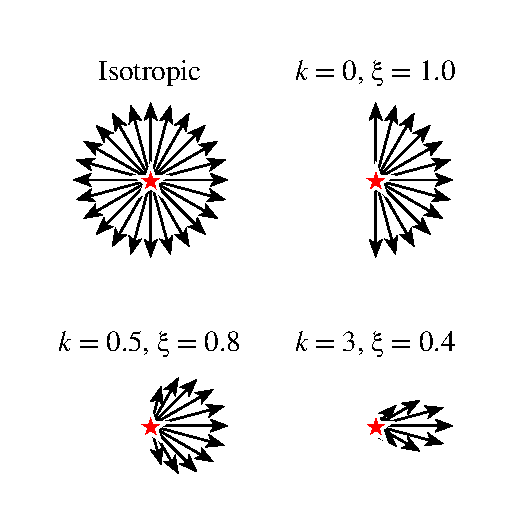
\includegraphics[width=0.5\linewidth]{./Figures/anisotropic-arrows}
  \caption{Representación esquemática de vientos con diferentes anisotropías: Arriba izquierda: Viento isotrópico esférico. Arriba derecha: viento isotrópico hemisférico. Abajo: Vientos anisotrópicos donde el parámetro $k$ indica el grado de anisotropía (ver capítulo \ref{chap:hipersonica}). $\xi = \frac{2}{k+2}$ es un parámetro introducido por conveniencia en el apéndice \ref{app:alatude-derivation}.}
    \label{fig:isotropic-aniso}
\end{figure}
\begin{figure}
  \centering
  \begin{tabular}{lr}
    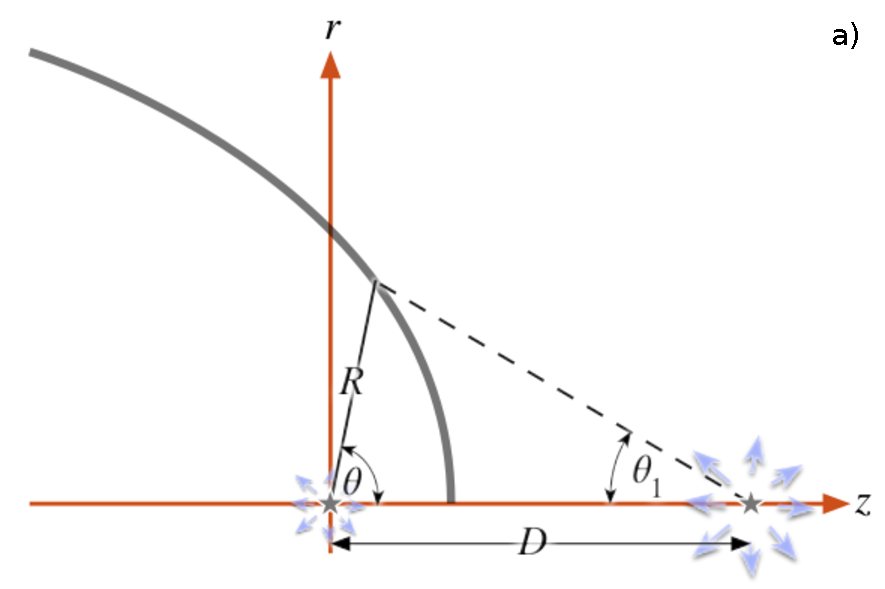
\includegraphics[width=0.45\linewidth]{./Figures/bowshock-crw-variables} &
    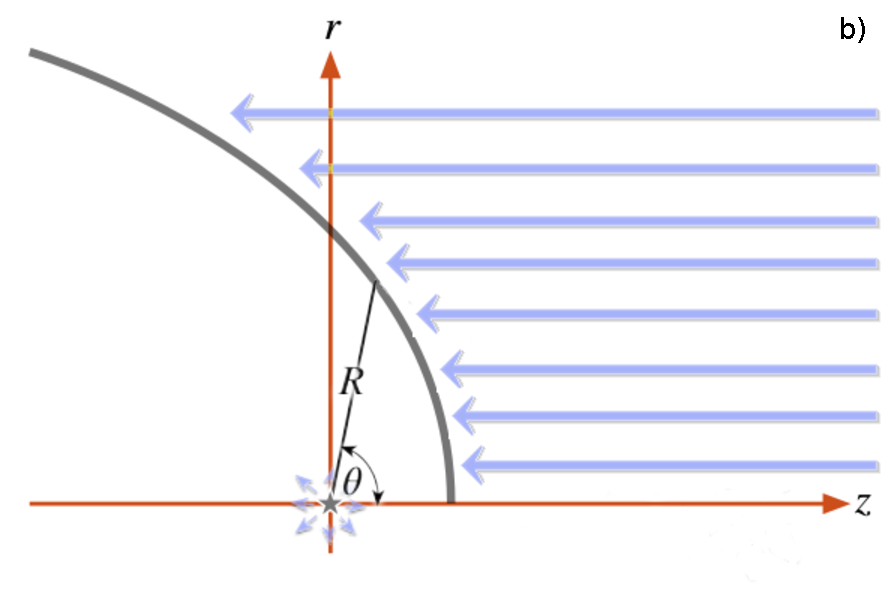
\includegraphics[width=0.45\linewidth]{./Figures/wilkinoid}
  \end{tabular}
  \caption{a) Representación esquemática del problema de interacción de dos vientos esféricos: Dos fuentes separadas por una distancia $D$ emiten un viento radial que forma un choque de proa a una distancia $R$ del origen. El sistema tiene geometría cilíndrica siendo el eje $z$ el eje de simetría. La forma del choque es función únicamente del ángulo polar $\theta$, medido a partir del origen. Otro ángulo que es de utilidad es $\theta_1$, que corresponde al ángulo polar medido a partir de la posición de la otra fuente. Cuando el viento interior tiene densidad constante y es esférico, denominamos al choque resultante como ``cantoide'', mientras que si su densidad sigue una ley de potencias de $\cos\theta$, con índice $k$, será un choque ``ancantoide''. b) Representación esquemática de la interacción de un choque esférico e isotrópico con una corriente plano--paralela de densidad y velocidad constantes. El choque resultante es en este caso de tipo ``wilkinoide''.}
    \label{fig:crw-esquema}
\end{figure}

\section{Parámetros Fundamentales}
\label{sec:fundamental-parameters}
El valor mínimo de $R(\theta)$, bajo las condiciones ya mencionadas, ocurre en el ápex $(\theta=0)$, y lo denotamos como $R_0$. Bajo la condición de estado estacionario, la condición de equilibrio de presión ram entre ambos vientos implica que:

\begin{align}
  \frac{R_0}{D} = \frac{\beta^{1/2}}{1 + \beta^{1/2}}
\end{align}

Donde $\beta$ es el cociente de la tasa de momentos entre los vientos en interacción. La tasa de pérdida de masa del viento interior es $\dot{M}_w$ y su velocidad terminal es $v_w$ y para el viento exterior estas cantidades son $\dot{M}_{w1}$ y $v_{w1}$. De esta forma, la tasa de momentos es:

\begin{align}
  \beta = \frac{\dot{M}_w v_w}{\dot{M}_{w1} v_{w1}} \label{eq:beta-def}
\end{align}

En el caso de que el viento exterior sea una corriente plano--paralela (wilkinoide), puede verse como el límite donde $D\to\infty$, lo que implica que a su vez se trata del límite donde $\beta\to 0$.
%correspondería al caso en que $\beta\to 0$, entonces $D$ deja de ser un parámetro relevante, ya que técnicamente $D\to\infty$.


\section{Planitud y ``Alatud''}
\label{sec:char-rad}

$R_0$ nos indica la escala del choque de proa, pero para caracterizar su forma utilizamos parámetros adicionales, mostrados en la figura \ref{fig:char-radii}. El radio perpendicular $R_{90}$ se obtiene evaluando la función $R(\theta)$ en $\theta=\pi/2$, mientras $R_c$ es el radio de curvatura medido en la posición del ápex. En el apéndice \ref{app:math-curvature-radius} mostramos que en el caso general en coordenadas cartesianas el radio de curvatura de una curva plana genérica $\vec{\sigma}(t)$ continua y derivable cuyas componentes son $(x(t), y(t))$ viene dado por:%que en coordenadas cilíndricas se calcula como sigue (ver apéndice \ref}):

\begin{align}
  R_c(t) = \frac{\left(\dot{x}^2 + \dot{y}^2\right)^{3/2}}{\left|\ddot{x}\dot{y} - \ddot{y}\dot{x}\right|} \label{eq:Rc-general-xy} 
\end{align}
donde $\dot{x}$ y $\dot{y}$ son las derivadas de $x$ e $y$ respecto a un parámetro adimensional $t$.

Haciendo la transformación a coordenadas polares con las ecuaciones (\ref{eq:polar-to-x}, \ref{eq:polar-to-y}) y con $\theta=t$, y evaluando el resultado en $\theta=0$ encontramos que:

\begin{align}
  R_c = \frac{R^2_0}{R_0 - R_{\theta\theta, 0}} \label{eq:generic-Rc}
\end{align}

donde $R_{\theta\theta, 0}\equiv \frac{d^2R}{d\theta^2}$ evaluado en $\theta = 0$.

Una forma simple de obtener el radio de curvatura es haciendo una expansión Taylor para la función $R(\theta)$ como sigue:

\begin{align}
  R(\theta) \simeq R_0 + \frac{1}{2}R_{\theta\theta, 0}\theta^2 + \mathcal{O}(\theta^4) \ref{eq:R-poly}
\end{align}
y hacer un ajuste polinomial a $R(\theta)$ para $|\theta| < \Delta\theta$ y determinar $R_0$ y $R_{\theta\theta, 0}$ de los primeros coeficientes del ajuste, y posteriormente $R_c$ a partir de la ecuación \ref{eq:generic-Rc}. $\Delta\theta$ es el rango del ángulo polar dentro del cual se puede hacer el ajuste. $\Delta\theta = 30^\circ$ es una buena opción.
%Las cantidades medibles que nos ayudan a caracterizar un choque de proa las llamamos ``Radios característicos'' (ilustrados en la figura \ref{fig:char-radii}):
%\begin{itemize}
%\item Radio en dirección perpendicular al ápex. Denotado como $R_{90}$
%\item Radio de curvatura en el ápex. Denotado como $R_c$. En el apéndice \ref{app:math-curvature-radius} se muestra el procedimiento para obtener este radio para una curva genérica continua y derivable.
%\end{itemize}

\begin{figure}
  \centering
  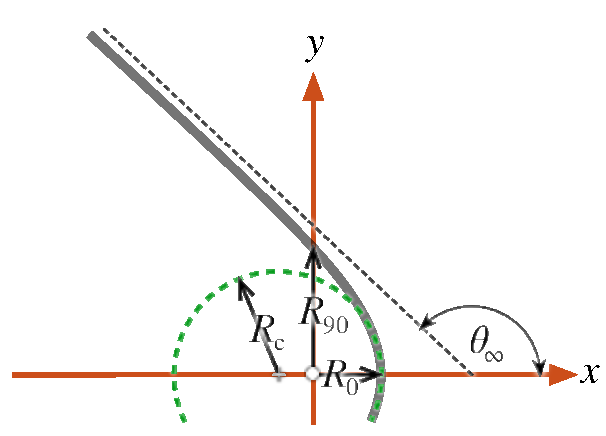
\includegraphics[width=0.5\linewidth]{./Figures/characteristic-radii}
  \caption{Representación esquemática de los radios característicos de un choque de proa}
  \label{fig:char-radii}
\end{figure}
Un último parámetro es el ángulo asintótico de apertura de las alas, denotado como $\theta_\infty$. Sin embargo, esta medida solo aplica para choques cuyas alas son asintóticamente cónicas, y aún para éstos en la mayoría de los casos es dificil de medirlo debido a que el ángulo polar $\theta$ tiende al valor asintótico muy lentamente y además la emisión de las alas es bastante débil. Por otro lado, los radios característicos $(R_0, R_c, R_{90})$ son medibles observacionalmente en la mayoría de los casos. A partir de éstos, podemos determinar dos parámetros adimensionales llamados ``planitud'' y ``alatud''. El primero de éstos es una medida de qué tan plano es el choque de proa en la nariz o ``apex'', y lo denotamos con la letra griega $\Pi$, mientras que el segundo es una medida de qué tanto se abren las alas del choque de proa, y lo denotamos con la letra griega $\Lambda$. Ambos parámetros se definen a continuación:

\begin{align}
  \Pi \equiv \frac{R_c}{R_0} \label{eq:planitude}\\
  \Lambda \equiv \frac{R_{90}}{R_0} \label{eq:alatude}
\end{align}

\section{Cuádricas de Revolución}
\label{sec:quadrics}
\newcommand\Sin{\ensuremath{\mathcal{S}}}
\newcommand\Cos{\ensuremath{\mathcal{C}}}
\newcommand\Cot{\ensuremath{\mathcal{T}}}
\newcommand\Q{\ensuremath{\mathcal{Q}}}
\newcommand\fQi{\ensuremath{f_{\scriptscriptstyle \Q, i}}}
% En el caso general es difícil encontrar la forma aparente para un choque de proa siguiendo el formalismo desarrollado en la sección anterior, por lo que optamos por aproximar la forma éstos con una de las superficies más simples: las \textit{cuádricas de revolución}, que son superficies de revolución de las curvas cónicas. Dado el modelo general descrito en la \S \ref{sec:Modelo-generico}, haremos algunas restricciones para las superficies cuádricas que utilizaremos en este trabajo:

Un tipo de superficies relevante y matemáticamente simple son las \textit{Cuádricas de Revolución} \citep{Goldman:1983a, Gfrerrer:2009a}, que son superficies de revolución de las secciones cónicas (círculo, elipse, parábola e hipérbola). Estas superficies son muy flexibles y pueden ser una aproximación muy útil a choques de proa con formas más complejas.

La forma de la cuádrica en el plano $xy$ se muestra en la figura \ref{fig:conics} para elipses e hipérbolas, respectivamente. La sección cónica en sí se describe con dos parámetros, que son los semi-ejes $a$ y $b$. Sin embargo, la curva puede desplazarse a lo largo del eje $x$, de manera que el radio en el ápex $R_0$ sea independiente de $a$ y $b$, para eso utilizamos un tercer parámetro denominado $x_0$ que nos indica el desplazamiento del centro de la curva respecto al origen.

%\begin{itemize}
%  \item El eje focal se encuentra alineado con el eje $x$
%  \item La posición del foco de la superficie cuádrica no necesariamente coincide con la posición de la fuente
%  \item En el caso de las hipérbolas, solo tomamos una de las ramas de ésta.
%\end{itemize}
De esta manera hacemos la representación paramétrica de las curvas cónicas en términos de un parámetro adimensional denotado con la letra $t$:
\begin{align}
  x &= x_0 + \sigma a\Cos(t) \\
  y &= b\Sin(t) 
\end{align}
Donde:
\begin{align}
  \Cos(t), \Sin(t) &=\left\lbrace
  \begin{array}{lr}
    \cos{t}, \sin t & \mathrm{elipses}\\
    \cosh{t}, \sinh{t} & \mathrm{hipérbolas}       
  \end{array}\right. \\
  \sigma &= \left\lbrace
  \begin{array}{lr}
    +1 & \mathrm{elipses} \\
    -1 & \mathrm{hipérbolas}
  \end{array}\right. \\
  x_0 &= R_0 -\sigma a \label{eq:x0} 
\end{align}
%Donde $a$ y $b$ representan la longitud de los semi-ejes de la cónica en cuestión (Figura \ref{fig:conics}) y $x_0$ representa la distancia entre el centro de la cónica y el origen. En esta figura representamos 
Por otro lado, la forma polar del choque de proa $R(\theta)$ viene dada por:

\begin{align}
  \tan\theta &= \frac{b\Sin(t)}{a\Cos(t) + x_0} \label{eq:t-th-conversion} \\
  R &= \left(\left(a\Cos(t) + x_0\right)^2 + b^2\Sin^2(t)\right)^{1/2} 
\end{align}
El tipo de cónica lo podemos caracterizar mediante el parámetro $\Q$, donde:
\begin{align}
  \Q \equiv \sigma\frac{b^2}{a^2} \label{eq:conic-parameter-a-b}
\end{align}
Para las superficies abiertas (hiperboloides) tenemos que $\Q < 0$, mientras que para las superficies cerradas tenemos que $\Q > 0$. Casos particulares son la esfera $\Q = 1$ y el paraboloide $\Q = 0$. De manera equivalente se puede definir el ángulo $\theta_Q$ como sigue:
\begin{align}
  \tan\theta_Q = \sigma \frac{b}{a} \label{eq:thc}
\end{align}
Este ángulo se relaciona con la excentricidad de las cónicas (y que sustituye a esta última en este trabajo) como se muestra a continuación:
\begin{align}
  \tan\theta_Q = \sigma\sqrt{\left|1-e^2\right|}
\end{align}
\begin{figure}
  \centering
  \begin{tabular}{cc}
    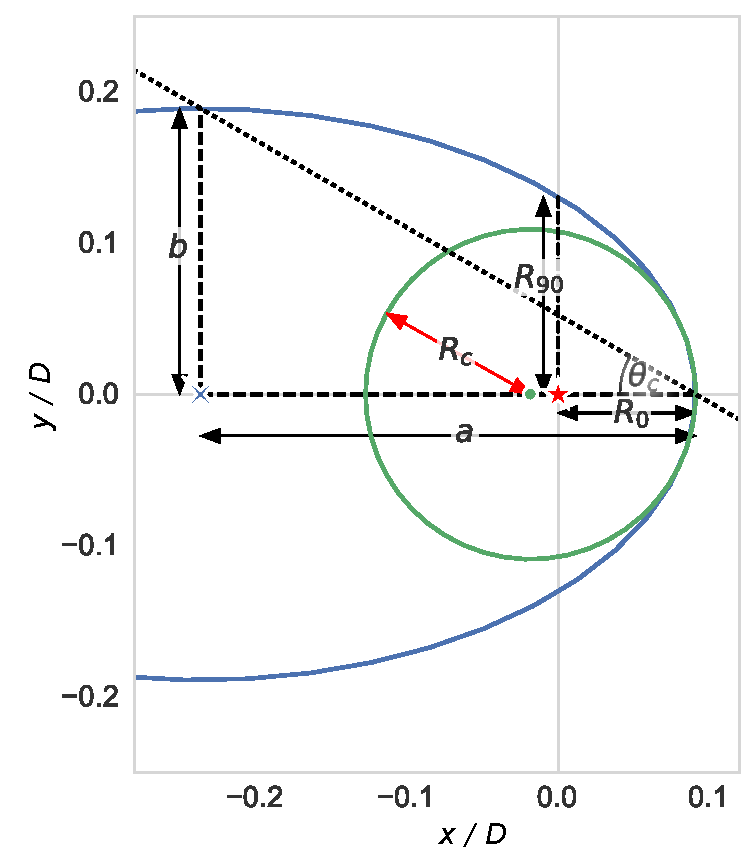
\includegraphics[width=0.4\linewidth]{./Figures/ellipse_edited} &
    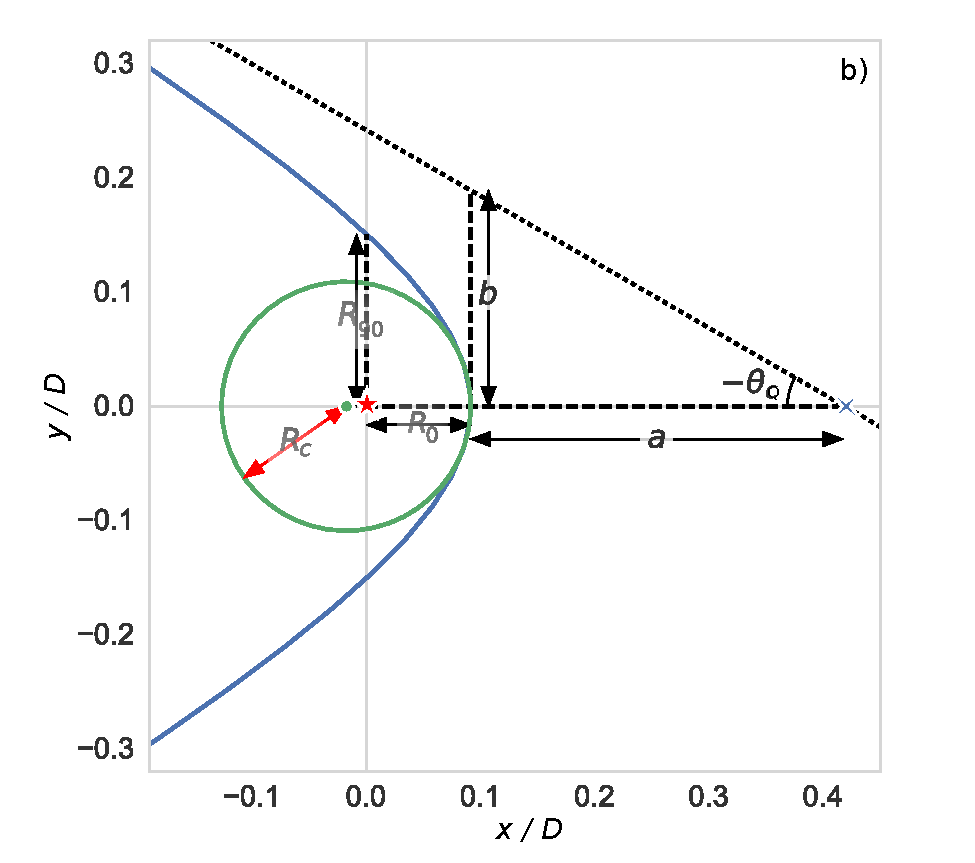
\includegraphics[width=0.5\linewidth]{./Figures/hyperbola_edited}
  \end{tabular}
  \caption{Representación esquemática de: a) Elipse. Y, b) Hipérbola. En ambos casos se ilustran los parámetros relevantes de éstas y los radios característicos}
  \label{fig:conics}
\end{figure}

\begin{figure}
  \centering
  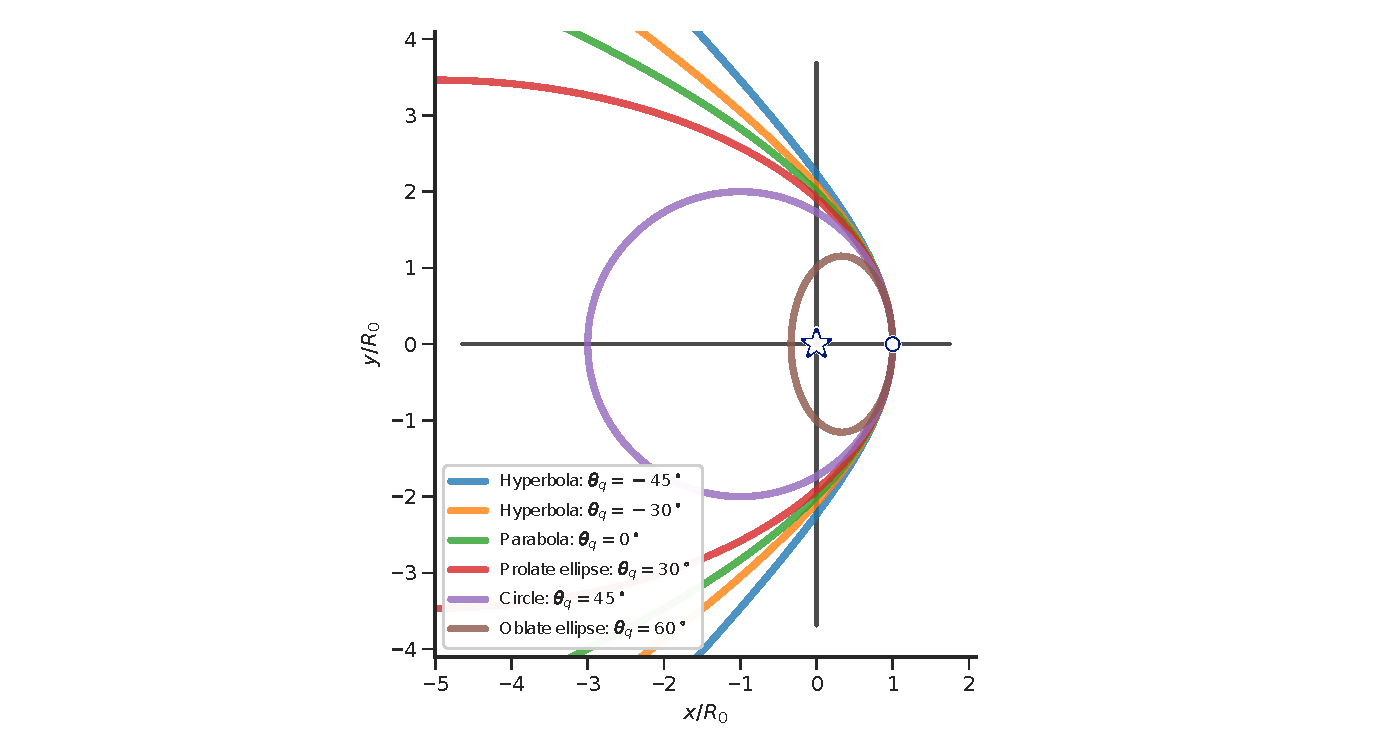
\includegraphics[width = \linewidth]{./Figures/conic1}
  \caption{Familia de curvas cónicas, donde el valor del parámetro $\theta_Q$ varía desde $\theta_Q < 0$ (hipérbolas) hasta $\theta_Q > 0$ (elipses). Casos especiales son $\theta_Q = 0$ (parábola) y $\theta_Q = 45^\circ$ (círculo). Este parámetro sustituye en este trabajo a la excentricidad.}
  \label{fig:conics-family}
\end{figure}
El conjunto de parámetros $(a, x_0, \Q)$ es suficiente para caracterizar a nuestras cuádricas de revolución: $\Q$ nos indica el tipo de cónica, $a$ establece la escala y $x_0$ el desplazamiento del centro a lo largo del eje $x$. Sin embargo, para futuras aplicaciones tanto a modelos de interacción de vientos como a observaciones (capítulos \ref{chap:hipersonica} y \ref{chap:proplyds}) nos sería util hacer la caracterización mediante los parámetros $(R_0, \Pi, \Lambda)$ (ver \S \ref{sec:char-rad}). Las equivalencias entre los dos conjuntos de parámetros los calculamos a continuación:
\begin{align} 
  R_c &= \frac{b^2}{a} = a|\Q|\label{eq:R-curv-conic}\\
  R^2_{90} &= b^2\sigma\left(1 - \frac{x^2_0}{a^2}\right) = \Q\left(a^2 - x^2_0\right)\label{eq:R90-conic} 
\end{align}
Combinando las ecuaciones (\ref{eq:planitude}, \ref{eq:alatude}, \ref{eq:x0}, \ref{eq:conic-parameter-a-b}, \ref{eq:R-curv-conic}, \ref{eq:R90-conic}), obtenemos lo siguiente:

\begin{align}
  R_0 &= x_0 + \sigma a \label{eq:R0}\\
  \Pi &= \frac{a|\Q|}{x_0 + \sigma a} = \frac{a\Q}{\sigma\left(x_0 + \sigma a\right)} = \frac{a\Q}{\left(a + \sigma x_0\right)}\label{eq:quadric-planitude}\\
  \Lambda &= \left(\Q\frac{a-\sigma x_0}{a + \sigma x_0}\right)^{1/2}
\end{align}

De aquí podemos escribir el parámetro de las cuádricas $\Q$ en términos de la planitud y la alatud:

\begin{align}
  \Q = 2\Pi - \Lambda^2 \label{eq:quadric-parameter-pi-lambda}
\end{align}

Por tanto, el signo de $2\Pi - \Lambda^2$ determina si una cuádrica es esferoidal o hiperboloidal. En la figura \ref{fig:conics-family} mostramos como, para planitud constante, podemos tener una familia de cónicas variando únicamente la alatud, y por consiguiente, el parámetro $\Q$.

\section{Proyección en el Plano del Cielo}
\label{sec:projection}

Para un choque de proa que es la vez geométricamente delgado y ópticamente delgado, únicamente se observa el borde de éste por
abrillantamiento al limbo, por lo tanto, su orientación respecto a la línea de visión modifica su forma respecto a la forma real del
choque. Para ello, rotamos el sistema de referencia del choque de proa en coordenadas cartesianas, denotado por $(x, y, z)$, por un ángulo que llamamos \textit{inclinación}, denotado por $i$, en el plano $xz$. La inclinación está definida de modo que cuando $i=0^\circ$ el eje de simetría del choque es perpendicular a la línea de visión, es decir, lo observamos ``de canto''. Y cuando $i = 90^\circ$ el eje desimetría es paralelo a la línea de visión, es decir, que lo observamos ``de frente''. De este modo la transformación entre el sistema de refencia del choque y el sistema de referencia del plano del cielo, denotado por $(x', y', z')$ queda como sigue:
\begin{align}
  \left(
  \begin{array}{c}
    x' \\ y' \\ z'
  \end{array}
  \right) = \mathbf{A}_y(i)
  \left(
  \begin{array}{c}
    x \\ y \\ z
  \end{array}
  \right) =
  \left(
  \begin{array}{c}
    x\cos i - z\sin i \\ y' \\ z\cos i + x\sin i
  \end{array}
  \right)
  \label{eq:rotation}
\end{align}

Donde $\mathbf{A}_y(i)$ está definida por la ecuación (\ref{eq:y-matrix}) en el apéndice \ref{app:matrix}.

Por otro lado, la forma tridimensional del choque de proa viene dado por una rotación alrededor del eje $x$ utilizando la matriz de rotación $\mathbf{A}_x(\phi)$ (ecuación \ref{eq:x-matrix}) sobre las ecuaciones (\ref{eq:polar-to-x}, \ref{eq:polar-to-y}):
\begin{align}
  \left(
  \begin{array}{c}
    x \\ y \\ z
  \end{array}
  \right) = \mathbf{A}_x(\phi)\left(
  \begin{array}{c}
    R(\theta)\cos\theta \\ R(\theta)\sin\theta \\ 0
  \end{array}
  \right)
  = \left(
    \begin{array}{c}
      R(\theta)\cos\theta \\
      R(\theta)\sin\theta\cos\phi \\
      R(\theta)\sin\theta\sin\phi
    \end{array}
    \right)
\end{align}
La relación entre ambos sistemas de referencia se ilustra en la figura \ref{fig:reference}.
\begin{figure}
  \centering
  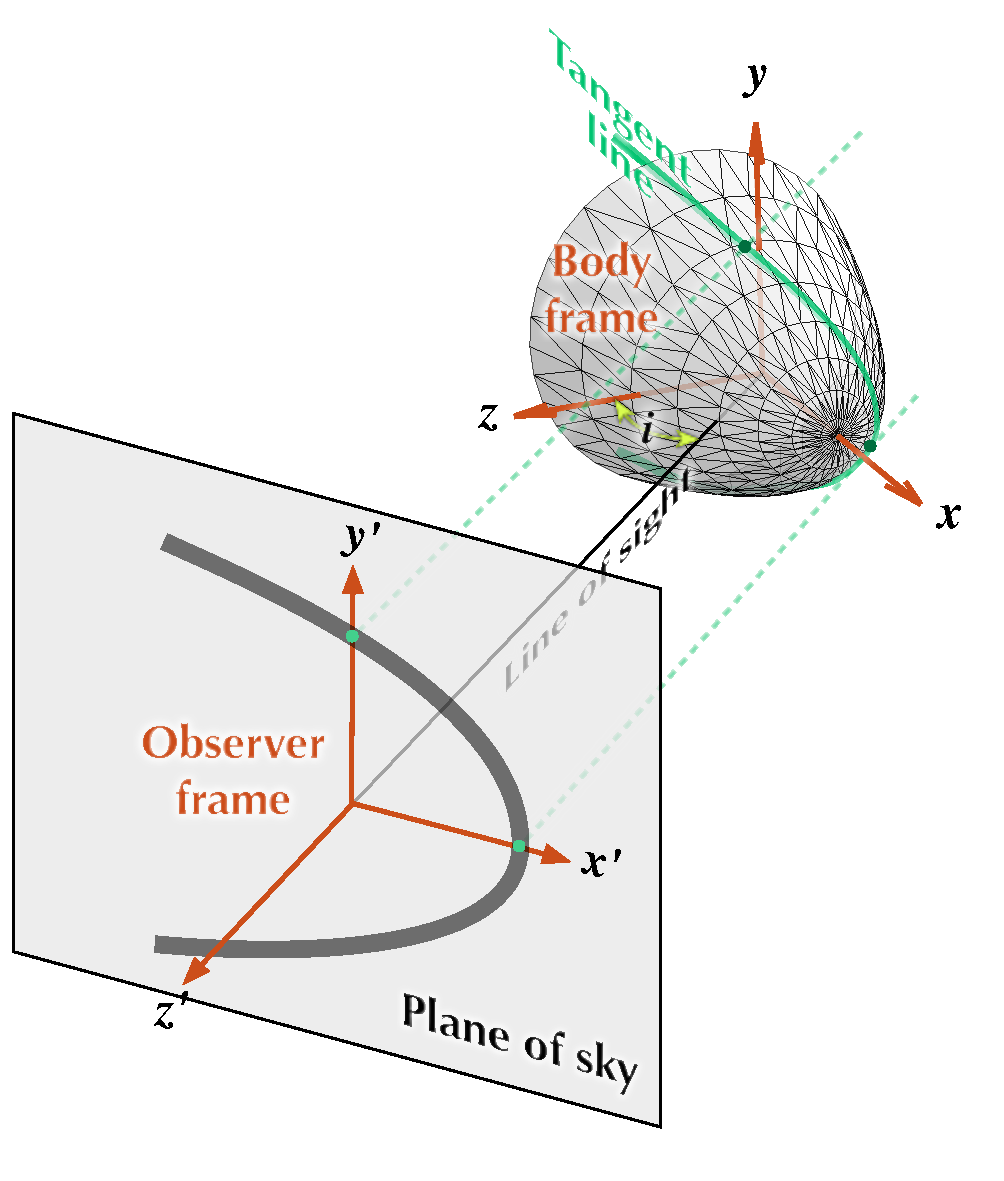
\includegraphics[width=0.5\linewidth]{./Figures/projection-pos}
  \caption{Sistema de referencia del choque vs sistema de referencia del plano del cielo. Los ejes $x'$ y $y'$ se encuentran en el plano del cielo, mientras el eje $z'$ es paralelo a la línea de visión. Solo la región del choque cuya tangente sea paralela a la línea de visión será visible por abrillantamiento al limbo.}
  \label{fig:reference}
\end{figure}

\subsection{Vectores normal y tangente a la superficie}

Definimos los vectores $\hat{n}$ y $\hat{t}$, como los vectores normal y tangente a la superficie, respectivamente para $\phi$ constante. En el caso $\phi = 0$ (figura \ref{fig:unit-vec}), ambos vectores se encuentran en el plano $xy$ y es fácil mostrar que:
\begin{align}
  \hat{t}_0 =
  \left(
  \begin{array}{c}
    -\cos\alpha \\
    \sin\alpha \\
    0
  \end{array}
  \right)
  \quad \mathrm{y} \quad
  \hat{n}_0 =
  \left(
  \begin{array}{c}
    \sin\alpha \\
    \cos\alpha \\
    0
  \end{array}
  \right)
  \label{eq:unit-vec}
\end{align}
Donde:
\begin{align}
  \tan\alpha = -\frac{dy}{dx} = \frac{1+\omega\tan\theta}{\tan\theta-\omega}
\end{align}
y:
\begin{align}
  \omega(\theta) = -\frac{1}{R}\frac{dR}{d\theta} 
\end{align}
Para $\phi \neq 0$, basta con hacer una rotación de las ecuaciones (\ref{eq:unit-vec}) alrededor del eje $x$ utilizando la matriz de rotación $\mathbf{A}_x(\phi)$:

\begin{align}
  \hat{n} &= \mathbf{A}_x(\phi)\hat{n}_0 =
 \left(
  \begin{array}{c}
    \sin\alpha \\
    \cos\alpha\cos\phi \\
    \cos\alpha\sin\phi
  \end{array}
  \right) \quad
    \hat{t} &= \mathbf{A}_x(\phi)\hat{t}_0 =
 \left(
  \begin{array}{c}
    -\cos\alpha \\
    \sin\alpha\cos\phi \\
    \sin\alpha\sin\phi
  \end{array}
  \right)
\end{align}

\begin{figure}
  \centering
  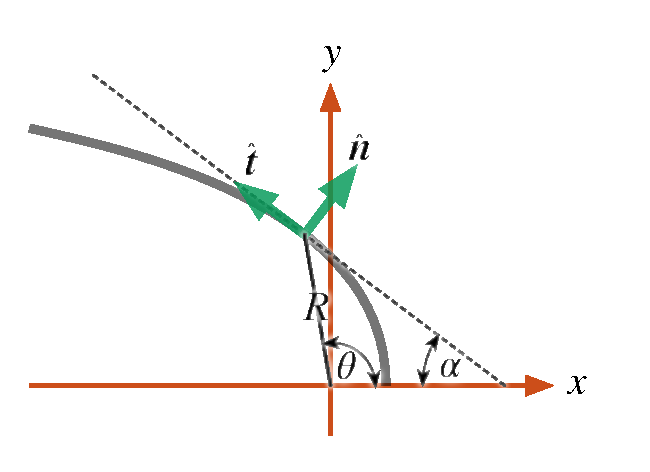
\includegraphics[width=0.6\linewidth]{./Figures/bowshock-unit-vectors}
  \caption{Vectores unitarios normal y tangente a la superficie $R(\theta)$
    en un plano de azimuth $\phi$ constante.}
    \label{fig:unit-vec}
\end{figure}

\subsection{Línea tangente}
\label{sec:tangent-line}
Debido a que el choque es ópticamente delgado y geométricamente delgado, solo la región del choque cuya tangente sea paralela a la
línea de visión será visible. Esto corresponde a una curva que denominamos \textit{línea tangente}, que debe cumplir con la siguiente
condición:
\begin{align}
  \hat{n}\boldsymbol{\cdot} \hat{z}' = 0
\end{align}
Denotamos como $\phi_T$ al ángulo azimutal que cumple la condición anterior para una inclinación dada, en función del ángulo polar $\theta$:
\begin{align}
  \sin\phi_T = -\tan i\tan\alpha = \tan i~\frac{1+\omega\tan\theta}{\omega-\tan\theta}
  \label{eq:phi-tan}
\end{align}
De esta manera, la forma de la línea tangente del choque de proa, a la que llamamos \textit{forma proyectada} viene dada por:
\begin{align}
  \left(
  \begin{array}{c}
    x'_T \\
    y'_T \\
    z'_T
  \end{array}
  \right) =
  R(\theta)\left(
  \begin{array}{c}
    \cos\theta\cos i - \sin\theta\sin\phi_T\sin i \\
    \sin\theta\left(1-\sin^2\phi_T\right)^{1/2} \\
    \cos\theta\sin i + \sin\theta\sin\phi_T\cos i
  \end{array}
  \right) \label{eq:proj-shape}
\end{align}
En el caso general, $z'_T$ no es una función lineal de $x'_T$ y $y'_T$, por lo que la línea tangente no se encuentra en un plano. La forma aparente $(x'_T, y'_T)$  de la línea tangente también puede escribirse en coordenadas polares $(R', \theta')$, donde:
\begin{align}
  R'(\theta) = \left(x'^2_T + y'^2_T\right)^{1/2} \quad \mathrm{y} \quad \tan\theta' = \frac{y'_T}{x'_T}
  \label{eq:polar}
\end{align}
Es de notar a su vez que la ecuación (\ref{eq:phi-tan}) no tiene solución para valores arbitrarios de $\theta$ y de la inclinación, puesto que se requiere que $\left|\sin\phi_T\right| < 1$. Por tanto, la línea tangente solo existe para valores de $\theta$ tales que $\theta < \theta_0$ donde $\theta_0$ es el valor de $\theta$ en el eje de simetría de la línea tangente proyectada $(\theta'(\theta_0) = 0)$ y que se obtiene resolviendo la siguiente ecuación implícita:
\begin{align}
  \tan\theta_0 = \frac{|\tan i| + \omega(\theta_0)}{1 - \omega(\theta_0)|\tan i|}
  \label{eq:th-0}
\end{align}
Esto implica que si el choque de proa es suficientemente ``abierto'' $(\alpha > \alpha_{min})$, entonces para inclinaciones tales que
$|i| > 90^\circ - \alpha_{min}$ no existirá la línea tangente para ningún valor de $\theta$, es decir, el choque de proa se encontrará sufientemente ``de cara'' como para que ya no parezca un choque de proa para el observador.

\subsection{Planitud y Alatud proyectadas: caso general}

La forma del choque de proa en el sistema de de referencia del cielo $R'(\theta')$ es la que actualmente se observa, por tanto
es necesario definir los radios característicos $R'_0$ y $R'_{90}$, donde $R'_0$ es el radio del eje de simetría aparente y $R'_{90}$ es el radio aparente en la dirección perpendicular a $R'_0$. Es decir $R'_0 = x'_T(y'_t=0)$ y $R'_{90} = y'_t(x'_t = 0)$. Utilizando las ecuaciones (\ref{eq:phi-tan}) y (\ref{eq:proj-shape}) encontramos que:
\begin{align}
R'_0 = R(\theta_0)\cos(\theta_0 - |i|)\footnotemark
\label{eq:R0p}
\end{align}\footnotetext{Evaluando la ecuación (\ref{eq:phi-tan}) en $\theta=\theta_0$ con ayuda de la ecuación (\ref{eq:th-0}) encontramos que $\sin\phi_T(\theta_0) = -\frac{\tan i}{|\tan i|}$ por lo que al sustituir este resultado en la componente $x$ de la ecuación (\ref{eq:proj-shape}) encontramos que $R'_0 = R(\theta_0)\left(\cos\theta_0\cos i + \sin\theta_0\sin i\frac{\tan i}{|\tan i|\right)}$ que finalmente se reduce al resultado de la ecuación (\ref{eq:R0p})}
Donde $\theta_0$ es la solución de la ecuación (\ref{eq:th-0}), y
\begin{align}
  R'_{90} = R(\theta_{90})\sin\theta_{90}\left(1-\sin^2\phi_T(\theta_{90})\right)^{1/2}
  \label{eq:R90p}
\end{align}
donde $\theta_{90}$ es la solución de la siguiente ecuación implícita:
\begin{align}
  \cot\theta_{90} = \frac{1 - \left(1+\omega(\theta_{90})^2\sin^22i\right)^{1/2}}
  {2\omega(\theta_{90})\cos^2i}
  \label{eq:th90}
\end{align}

Por otro lado, el radio de curvatura aparente se obtiene a partir de la ecuación (\ref{eq:generic-Rc}) pero en el sistema de referencia primado:

\begin{align}
  R'_c = \frac{R'^2_0}{R'_0 - R'_{\theta'\theta', 0}} \label{eq:Rc-prime}
\end{align}

\subsection{Aplicación a las Cuádricas de Revolución}
\label{sec:pi-lambda-quadric}
El objetivo de esta sección es obtener la forma proyectada de las cuádricas de revolución, puesto que son una aproximación buena y mucho más sencilla a la forma real de un choque de proa. Para esto es conveniente utilizar un sistema de referencia donde el origen se ubica en el centro de la sección cónica:

\begin{align}
  (X, Y) = (x-x_0, y)
\end{align}
de esta manera, la forma de las cuádricas de revolución es:


\begin{align}
  \left(
  \begin{array}{c}
    X \\ Y \\ Z
  \end{array}
  \right) = \mathbf{A}_x(\phi)\left(
  \begin{array}{c}
    a\Cos(t) \\ b\Sin(t) \\ 0
  \end{array}
  \right)
  = \left(
    \begin{array}{c}
      a\Cos(t) \\
      b\Sin(t)\cos\phi \\
      b\Sin(t)\sin\phi
    \end{array}
    \right)
\end{align}

Siguiendo el procedimiento mostrado en la \S \ref{sec:projection} calculamos el ángulo azimutal $\phi$ que cumple con el criterio de ser tangente a la línea de visión: 

\begin{align}
  \sin\phi_T = \frac{b\Cos(t)}{a\Sin(t)}\tan i 
\end{align}
Ahora utilizamos la ecuación (\ref{eq:rotation}) para obtener la forma aparente de una cuádrica dada:
\begin{align}
  X'_T &= \frac{\Cos(t)}{a\cos i}\left(a^2\cos^2 i + \sigma b^2\sin^2 i\right)
  \label{eq:x-prime-proj}\\
  Y'_T &= b\Sin(t)\left(1 - \frac{b^2\Cos^2(t)}{a^2\Sin^2(t)}\tan^2 i\right)^{1/2}
  \label{eq:y-prime-proj}
\end{align}
Podemos mostrar que la forma proyectada de una sección cónica (elipse o hipérbola), es de la misma clase que la sección cónica original. Si ese fuera el caso, entonces podemos escribir las ecuaciones (\ref{eq:x-prime-proj}, \ref{eq:y-prime-proj}) de la siguiente manera:
\begin{align}
  X'_T &= a'\Cos(t') \label{eq:xtprime}\\
  Y'_T &= b'\Sin(t') \label{eq:ytprime}
\end{align}

Después de un poco de álgebra encontramos que nuestra suposición es consistente, con las siguientes equivalencias:

\begin{align}
  a' &= a\cos i \fQi \label{eq:a-prime}\\
  b' &= b \label{eq:b-prime}\\
  \Cos(t') &= \fQi \Cos(t)
\end{align}

Donde introducimos el factor de proyección de las cuádricas:
\begin{align}
  \fQi = \left(1 + \Q\tan^2i\right)^{1/2} \label{eq:Q-factor}
\end{align}


%Dos cantidades que nos van a ser de utilidad son los valores del parámetro $t$ que denominaremos $t_0$ y $t_{90}$ y son tales que $t'(t_0) = 0$ y $t'(t_{90}) = \frac{\pi}{2}$ o bien $y'_T(t_0) = 0$ y $x'_T(t_{90}) = 0$. De esta manera obtenemos las siguientes ecuaciones implícitas evaluando las ecuaciones (\ref{eq:x-prime-proj}) y(\ref{eq:y-prime-proj}) en $t=t_{90}$ y $t=t_0$ respectivamente:
%\begin{align}
%  \Cot(t_0) &= \frac{a}{b}\cot{i} = \frac{\cot{i}}{\left|\tan\theta_c\right|} %\label{eq:t0}\\
%  \Cos(t_{90}) &= -\frac{ax_0\cos^2{i}}{a^2\cos^2{i}\pm b^2\sin^2{i}} \label{eq:t90}
%\end{align}
Como ya demostramos que la forma proyectada de la línea tangente de una superficie cúadrica es una sección cónica del mismo tipo, entonces podemos determinar la forma proyectada reutilizando las ecuaciones (\ref{eq:R0}-\ref{eq:quadric-parameter-pi-lambda}) sustituyendo las cantidades no primadas por sus equivalentes primados. De esta manera, utilizando las ecuaciones (\ref{eq:conic-parameter-a-b}, \ref{eq:a-prime}, \ref{eq:b-prime}) encontramos que el parámetro de las cuádricas para la forma proyectada es:

\begin{align}
  \Q' = \frac{\Q}{\fQi^2 \cos^2 i}\label{eq:Q-prime}
\end{align}

Ahora regresamos al sistema de referencia centrado en la estrella:

\begin{align}
  (x'_T, y'_T) = (X'_T + x'_0, Y'_T)
\end{align}

donde el desplazamiento proyectado $x'_0$ es:

\begin{align}
  x'_0 = x_0\cos i
\end{align}
La proyección de la distancia al ápex viene dada por la versión primada de la ecuación (\ref{eq:R0}):
\begin{align}
  R'_0 &=  x'_0 + \sigma a'\\
  \implies \frac{R'_0}{R_0} &= \cos i\left[1 + \frac{\Pi}{\Q}\left(1 - \fQi\right)\right] \label{eq:R0p-R0-quad}
\end{align}eq;

Asimismo la planitud y la alatud proyectada pueden calcularse a partir de las ecuaciones (\ref{eq:quadric-planitude}, \ref{eq:quadric-parameter-pi-lambda}, \ref{eq:a-prime}, \ref{eq:Q-prime}):

\begin{align}
  \Pi' &= \frac{\Pi}{\left(R'_0/R_0\right)\fQi\cos i} \label{eq:quadrics-planitude-prime}\\
  \Lambda' &= \left(2\Pi' - \Q'\right)^{1/2} \label{eq:quadrics-alatude-prime}
\end{align}

En la figura \ref{fig:proj-L-P-vs-i} mostramos el comportamiento de la planitud y la alatud aparente con la inclinación para distintos valores del parámetro $\Q$ (color) y de la planitud $\Pi$ (grosor de la curva). Se puede observar que para las superficies elipsoidales $(\Q > 0)$, la planitud y alatud aparente tienden a $\Pi' = \Lambda' = 1$ conforme $i \to 90^\circ$. Esto se debe a que en este límite observamos la superficie de frente y vemos su sección transversal circular. En el caso del paraboloide la convergencia se da a $\Lambda' = \Pi' = 2$. Por otro lado, la planitud y alatud aparente divergen cuando $|i| \to i_{\mathrm{crit}} = 90^\circ - |\theta_\Q|$ debido a que, como ya mencionamos en la \S \ref{sec:tangent-line}, cuando $|i| > i_{\mathrm{crit}}$ ya no existe una línea tangente a la línea de visión y por tanto no se observaría abrillantamiento al limbo. También cabe destacar dos casos particulares: El esferoide confocal con planitud unitaria $(\Pi = 1)$ y el paraboloide confocal $(\Pi = \Lambda = 2)$. En estos dos casos su forma aparente no se ve afectada por la inclinación: para el esferoide confocal se puede mostrar fácilmente a partir de las ecuaciones (\ref{eq:Q-factor}, \ref{eq:Q-prime}, \ref{eq:R0p-R0-quad}-\ref{eq:quadrics-alatude-prime}) que si $\Q = 1$, $\Pi = 1$, entonces $\Pi'=1$, $\Lambda'=1$ y $\Q' = 1$, independientemente de la inclinación. De manera similar, tomando el límite de estas mismas ecuaciones cuando $\Q\to 0$ podemos estimar la planitud y alatud aparente del paraboloide, y para el caso particular donde $\Pi = 2$, se obtiene a su vez que $\Pi'=2$ independientemente de la inclinación.

\begin{figure*}
  \centering
  \begin{tabular}{lr}
    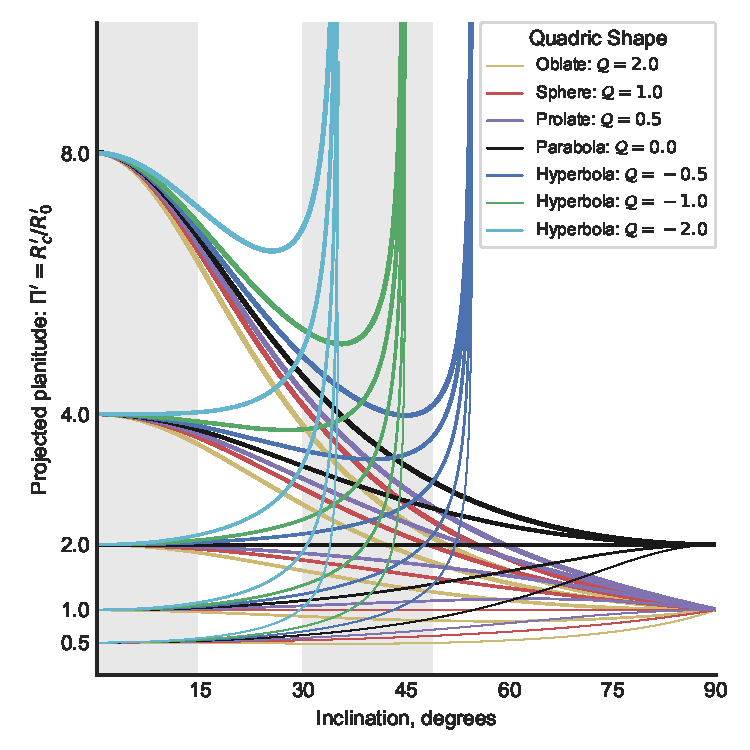
\includegraphics[width=0.5\linewidth]{./Figures/projected-Rc-vs-i} &
    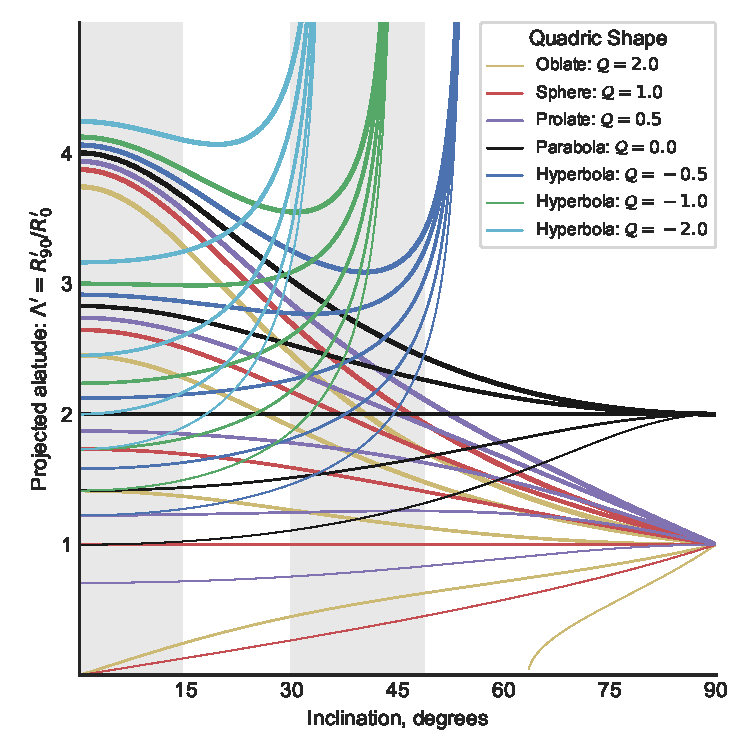
\includegraphics[width=0.5\linewidth]{./Figures/projected-R90-vs-i}
  \end{tabular}
  \caption{Efectos de la proyección sobre las cuádricas de revolución con la inclinación $|i|$. Los colores de las curvas representan variaciones en el parámetro $\Q$ de las cuádricas. El grosor de la curva indica el valor de la planitud intrínseca $\Pi$. Los rectángulos sombreados muestran cuartiles de $|\sin i|$ que se encuentran equitativamente poblados para una distribución isotrópica de orientaciones. (a) Planitud aparente $\Pi'$. (b) Alatud aparente $\Lambda'$}
  \label{fig:proj-L-P-vs-i}
\end{figure*}

\begin{figure}
  \centering
  \begin{tabular}{lr}
    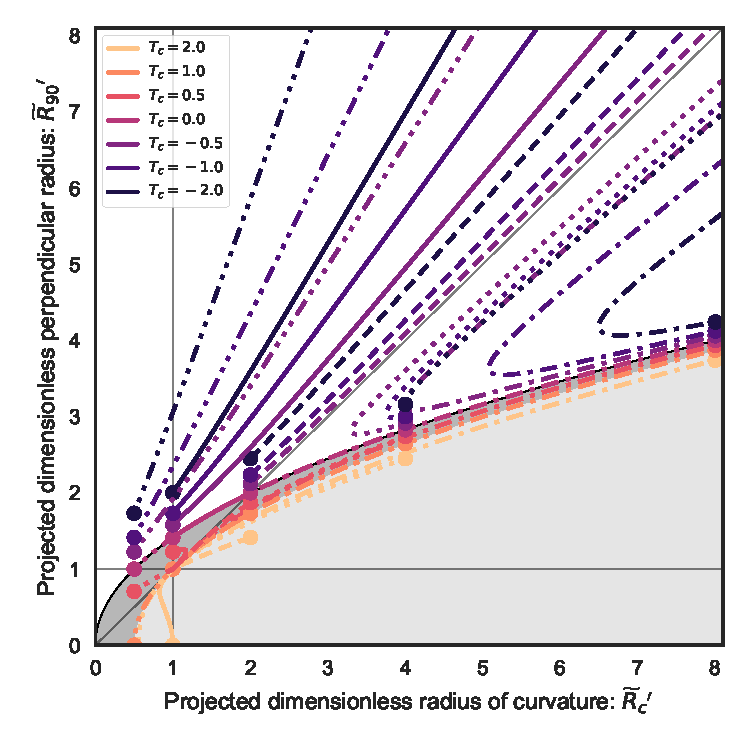
\includegraphics[width=0.5\linewidth]{./Figures/projected-R90-vs-Rc} &
    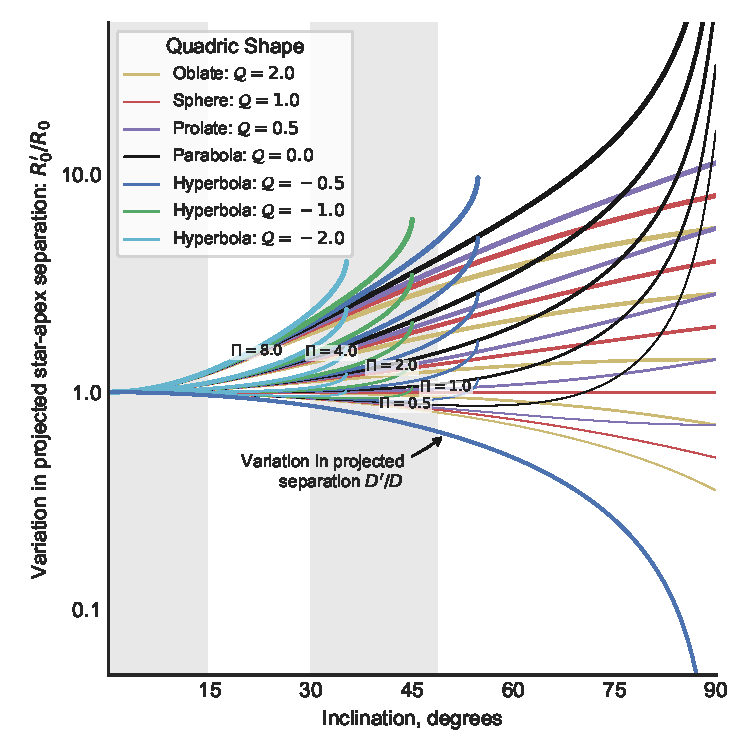
\includegraphics[width=0.5\linewidth]{./Figures/projected-R0-vs-i}
  \end{tabular}
  \caption{(a) Diagrama de diagnóstico $\Lambda'$ vs $\Pi'$ para diferentes tipos de cuádricas: esferoides oblatos (amarillo), esferoides (rojo), esferoides prolatos (morado), paraboloides (negro) e hiperboloides (azul, verde y turquesa). Cada punto de una curva representa un valor diferente de la inclinación, y se muestran explícitamente las inclinaciones múltiplos de $15^\circ$, con la forma de círculos rellenos. Las regiones sombreadas representan al tipo de cuádrica que mejor ajusta a los parámetros $(\Pi', \Lambda')$ cubiertos. La región clara para los hiperboloides, la región gris oscura para los esferoides prolatos y la región gris clara para los hiperboloides oblatos. La interfaz entre la región de hiperboloides y esferoides prolatos corresponde a los paraboloides y la región entre esferoides prolatos y oblatos a los esferoides. (b) Distacia proyectada $R'_0/R_0$ versus $|i|$.}
  \label{fig:Pip-Lambdap-diagnostic}
\end{figure}

En la figura \ref{fig:Pip-Lambdap-diagnostic}a observamos el diagrama de diagnóstico $\Pi'-\Lambda'$. Cada curva representa a una cuádrica de revolución siguiendo la misma convención que en la figura \ref{fig:proj-L-P-vs-i} para los valores de $\Q$ y $\Pi$ y variando la inclinación a lo largo de cada una de éstas, donde además el punto donde $i=0$ (cuádrica vista de canto) se marca con un punto. Las regiones sombreadas representan a cada clase de cuádrica, la zona superior más clara a los hiperboloides, la zona gris delgada a los elipsoides prolatos, la interfaz entre estas dos últimas a los paraboloides y la zona gris inferior a los elipsoides oblatos. Se puede observar que en ningún caso las curvas cruzan de una región a otra. También se observa de nuevo que las curvas elipsoidales convergen a $(\Pi', \Lambda') = (1, 1)$, las curvas hiperbólicas a $(\Pi', \Lambda') = (+\infty, +\infty)$ y las parabólicas a $(\Pi', \Lambda') = (2, 2)$. Asimismo en la figura \ref{fig:Pip-Lambdap-diagnostic}b observamos el comportamiento de la separación aparente estrella--ápex con inclinación. En este caso se observa que para inclinaciones pequeñas $(|i| < 30^\circ)$, esta separación depende muy poco del parámetro $\Q$, siendo más importante la planitud $\Pi$. Por otro lado, para inclinaciones mayores, la separación aparente se incrementa cada vez más rápido para cuádricas abiertas $(\Q \leq 0)$, mientras que para los elipsoides la separación es cada vez más lenta e incluso puede decrecer con inclinación.

\begin{figure}
  \centering
  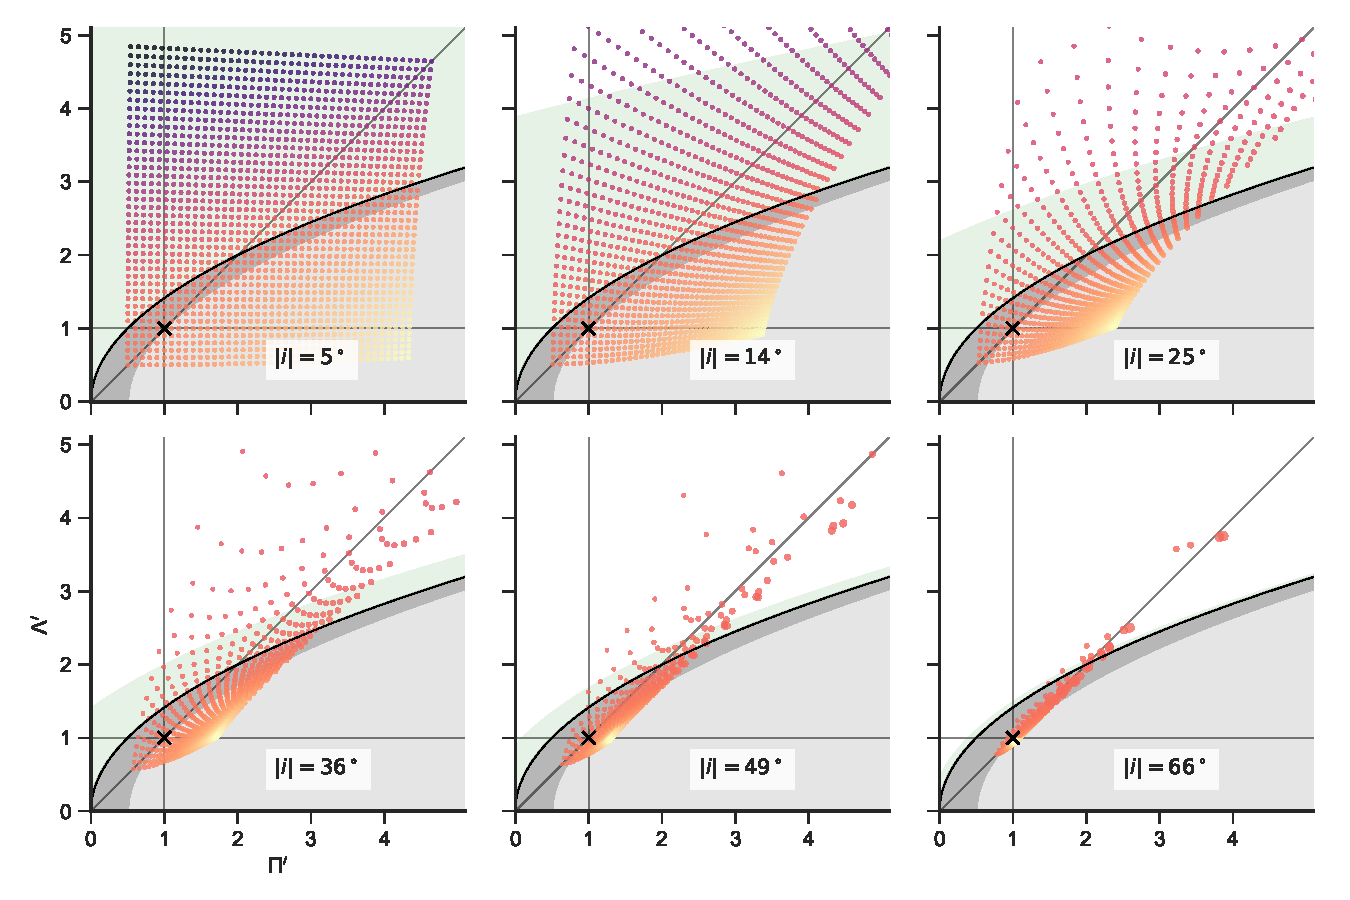
\includegraphics[width=\linewidth]{./Figures/projected-R90-Rc-snapshots}
  \caption{Efectos de la inclinación de la forma aparente de arcos cuádricos cuya planitud y alatud están uniformemente distribuídos en los rangos $\Pi = [0.5, 4.5]$, $\Lambda = [0.5, 4.5]$. En cada pánel se muestra la forma aparente incrementando la inclinación en intervalos iguales de $|\sin i|$. El collor representa el parámetro $\Q$, desde azul (menor valor de $\Q$, que representa formas más abiertas), pasando por naranja, hasta amarillo (elipsoides oblatos). El tamaño representa la distancia aparente estrella--ápex $R'_0/R_0$.}
  \label{fig:snapshots}
\end{figure}


En la figura \ref{fig:snapshots} mostramos una visión complementaria del análisis de la forma aparente con la inclinación. En esta figura se toman ``capturas'' de $(\Pi', \Lambda')$ en intervalos regulares de $\sin i$. Los valores de la planitud y alatud intrínseca están uniformemente distribuídos en los intervalos $\Pi = [0.5, 4.5]$ y $\Lambda = [0.5, 4.5]$, lo que nos da un cuadrado uniformemente distribuído de valores cuando $|i| = 0$, y que se va distorsionando conforme $|i|$ se incrementa. La escala de color representa el parámetro $\Q$, incrementándose dicho parámetro desde el azúl hasta el amarillo, pasando por el naranja, mientras que el tamaño del punto es proporcional a $R'_0/R_0$. Se puede observar que todos los puntos tienden a la línea $\Pi' = \Lambda')$ a altas inclinaciones, y que los puntos azules quedan fuera del rango de la gráfica. Esto es porque a altas inclinaciones, para las formas muy abiertas ya no existe la línea tangente a la línea de visión. De hecho, la región verde sombreada es la región para la cual aun existe la línea de visión para cada inclinación y se hace cada vez más pequeña conforme la inclinación aumenta. Esta figura es meramente cualitativa, puesto que no hay razón para esperar una distribución uniforme de planitud y alatud (en el siguiente capítulo encontramos que en el modelo de capa delgada no encontramos formas cuyo parámetro $\Q$ sea mayor a 1, por ejemplo).

% Utilizando las ecuaciones (\ref{eq:x0}), (\ref{eq:a-prime}) y (\ref{eq:b-prime}), utlizando la definición $D' = D\cos i$ e introduciendo la función $f(i;\theta_c)\equiv \left(1 \pm \tan^2\theta_c\tan^2i\right)^{1/2}$ obtenemos ecuaciones explícitas para los radios característicos en el sistema de referencia del plano del cielo en términos de la inclinación:
%\begin{align}
%  \frac{q'}{q} &= 1 \pm \tilde{R}_c\cot^2\theta_c\left(f(i;\theta_c) - 1\right) \\
%  \tilde{R}'_c &= \frac{\tilde{R_c}}{\cos^2if(i;\theta_c)\frac{q'}{q}} \label{eq:Rpc-quad}\\
%  \tan\theta'_c &= \frac{\tan\theta_c}{\cos if(i;\theta_c)} \label{eq:thcp-quad}\\
%  \tilde{R}'_{90} &= \left(\frac{2\tilde{R}_cf(i;\theta_c) \mp
%                    \tan^2\theta_c\frac{q'}{q}}{q'/q}\right)^{1/2}\frac{\sec %i}{f(i;\theta_c)}
%  \label{eq:Rp90-quad}
%\end{align}
%Cuando $\tilde{R}'_{90}$ es medible, entonces es posible hacer diagramas de diagnóstico como
%el de la figura \ref{fig:diagnostic} para comparar con observaciones, independientemente de cualquier modelo de choques de proa.
%\begin{figure}
%  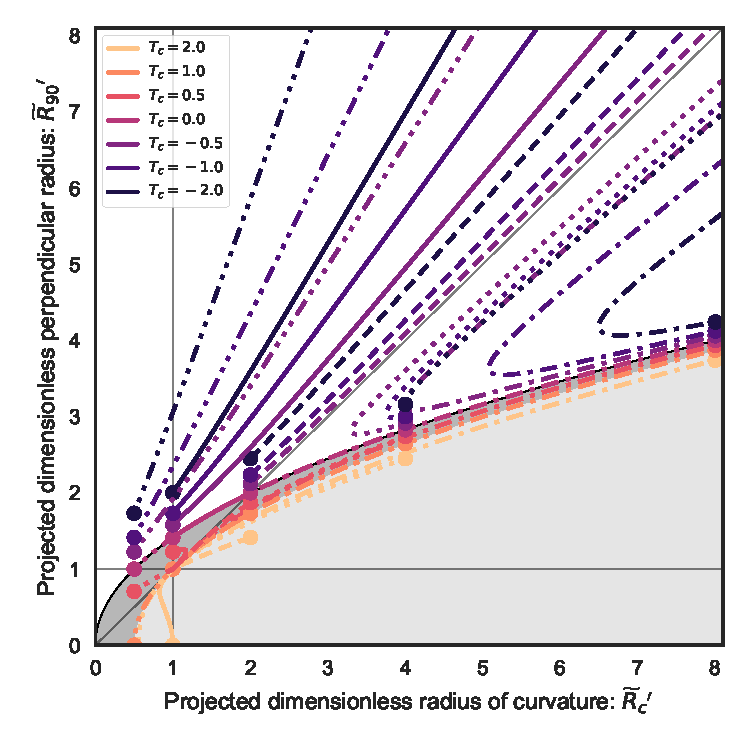
\includegraphics[width=0.5\linewidth]{./Figures/projected-R90-vs-Rc}
%  \caption{Diagrama de diagnóstico $\tilde{R}'_{90}$ vs $\tilde{R}'_c$ para las cuádricas de revolución. En la región sin sombrear se representan las superficies abiertas (hiperboloides, $\theta_c <0$), mientras que la región más oscura representa a elipsoides prolatos  $(0 < \theta_c < 45^\circ)$ y la región poco sombreada a elipsoides oblatos $(\theta_c > 45^\circ)$}
%  \label{fig:diagnostic}
%\end{figure}
